\section{本研究的意义和目的}

对于三维人体姿态估计,在不同的环境设定下有不同的输入,例如RGB单目输入、RGB双目输入、RGB与深度传感器输入和光学雷达(LiDAR)输入。目前很多人体姿态估计方法对视基于多摄像头或深度传感器的,并已经取得了不错的成果。然而深度传感器如Kinect\cite{kinect}成本较高,需要使用其特殊的设备采集数据。并且Kinect设备设光照影响较大,采集的深度范围有效,难以推广;多摄像头系统需要在固定的场景下,并且需要对多个相机之间的位置进行标定,难以推广到普通场景下;对于目前手机上常用的双目摄像头,其只能在较短距离内提供有效的双目的输入,在大多数距离范围内均只能当作单目摄像头处理。在生活中单目摄像头的产品最为常见,尤其是在网络视频传输、监控摄像头中,单目摄像头的使用便携性是远超过双目摄像头及其他的,并且成本也最低。这也就意味着基于廉价的单目摄像头的人体姿态估计更有应用前景,也就意味着单目RGB图像中进行人体姿态估计的研究更有价值。

基于视频的人体运动姿态分析有着广阔的引用场景,因此其吸引了越来越多研究者的兴趣。其应用领域主要表现在以下几个方面:

\begin{figure}[ht] \centering
    \subfigure[AR场景] { \label{fig:a}
    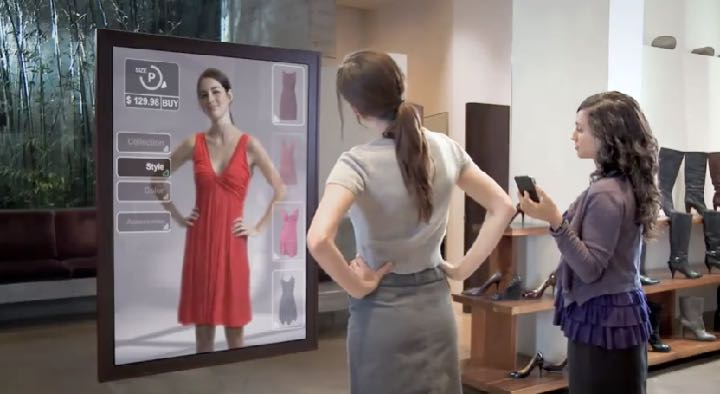
\includegraphics[height=0.15\columnwidth]{figure/background/ar.png}
    }
    \subfigure[人机交互] { \label{fig:appb}
    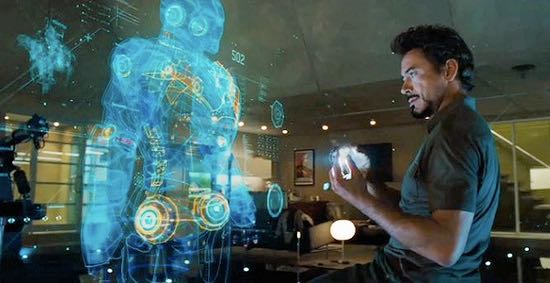
\includegraphics[height=0.15\columnwidth]{figure/background/hcl.png}
    }
    \subfigure[电影制作] { \label{fig:appc}
    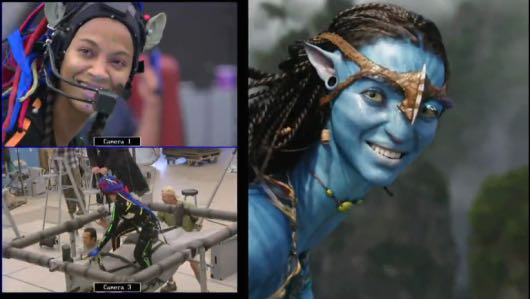
\includegraphics[height=0.15\columnwidth]{figure/background/movie.png}
    }
    \subfigure[娱乐游戏] { \label{fig:appd}
    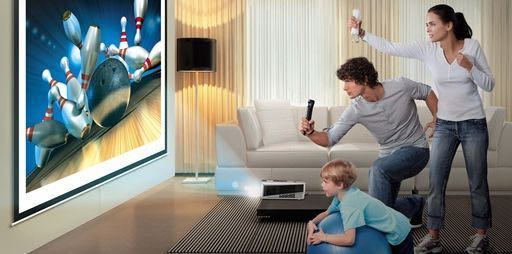
\includegraphics[height=0.15\columnwidth]{figure/background/gaming.png}
    }
    \subfigure[健康监护] { \label{fig:appe}
    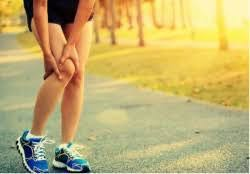
\includegraphics[height=0.15\columnwidth]{figure/background/health.png}
    }
    \subfigure[安防监控] { \label{fig:appf}
    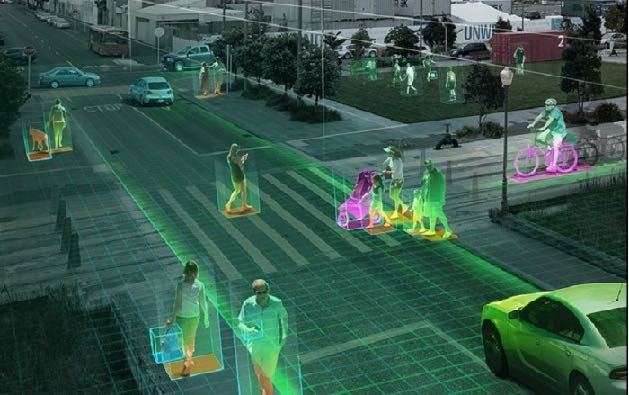
\includegraphics[height=0.15\columnwidth]{figure/background/surveil.png}
    }
    \caption{应用场景}
    \label{fig:appli}
\end{figure}


\textbf{虚拟现实和增强现实:}在虚拟环境中,人与虚拟角色进行的动作模拟,可以通过基于视频的人体姿态运动分析,给参与者提供更多的交互形式。计算机可以从视频中获取人体运动数据,可以使我们用新的虚拟人物或者动画角色替换原始视频中的人物,得到更好的效果。

\textbf{智能人机交互:}智能人机交互是指让目前的计算机摆脱键盘鼠标等传统交互设备的局限,通过人体运动等更为自然的方式直接用人类进行交互,使得计算机能像人与人之间的交流一样更自然便捷。这要求计算机能够更进一步地从面部表情、语言、身体动作去分析人的行为,而基于视觉分析的技术能够在语言干扰大的环境下提供更准确的输入。

\textbf{电影制作:}目前计算机进行电影和动画制作时,人物角色的动作、姿态的设计主要来源于运动捕捉设备的使用。传统的运动捕捉设备需要在人体身上贴满标签,该方法成本较高,使用麻烦。而基于视频的人体运动动作的获取,将给人体动画和游戏提供更加丰富的数据,并且也能大大降低运动捕捉系统的成本,提高制作效率。


\textbf{健康监护:}在临床上,通过获取患者的行走动作,利用计算机来分析其运动数据,有助于判断身体某部分的受伤情况或者畸形程度,从而帮助做出有效的治疗手段。而传统的运动分析系统大多采样专用的视频设备和计算机设备,价格昂贵,操作复杂,使用过程具有较高的专业性,因此不适合进行大范围的推广,难以在普通医院使用。因此采用普通电脑连接普通摄像机的人体运动姿态分析系统有着更广阔的应用场合和前景。

\textbf{智能安防监控:}目前监控摄像机在公共场所已经广泛存在,但是无法发挥其实时、积极的作用,大多数场合只能通过专门的工作人员监视显示器,以发现异常的事件。或者将监控视频保存,出现异常情况时,才调用监控记录进行查看,而这样又会占用大量存储设备,因此无法保留长时间记录。如果通过视频进行监视,通过计算机进行实时分析,通过检测并跟踪其中的人体运动,分析人体行为,当有异常情况发生时,系统能够及时警报,从而有效防止此类事件的发生。同时也可以减少大量雇佣人员的成本,以及购买存储设备的成本。


% \begin{figure}[ht]
%     \centering
%     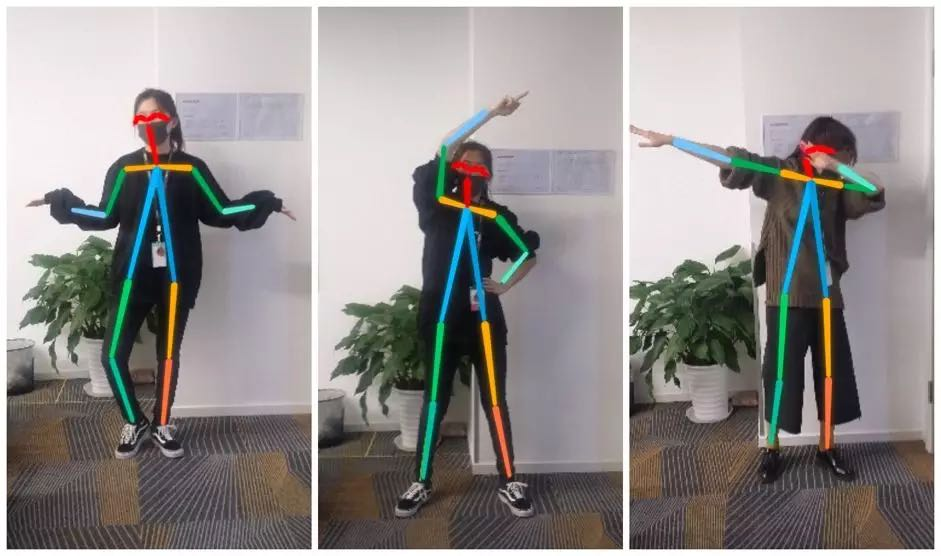
\includegraphics[width=.8\linewidth]{background/human}
%     \caption{\label{fig:cha3}二维人体姿态估计}
% \end{figure}

\section{主要研究内容}
本研究的重点在三维人体姿态估计,需要考虑的输入为单张图片输入、单目视频输入。并重点考虑在视频序列输入下的人体三维姿态估计,通过结合时间信息与空间信息,实现对人体姿态的更好的估计。

\section{技术路线}
% 要完成该项任务,需要分为多个步骤。分别是建立数据集、人体检测、二维人体姿态估计、三维人体姿态估计、结合人体几何模型的三维人体模型估计。
技术路线主要分为几个内容:
\begin{itemize}
    \item 数据集:通过开源数据集或自己的数据集,完成模型的测试及验证
    \item 人体检测:从图片中检测出人体的位置
    \item 二维人体姿态估计:从图片中获取人体的二维关键点的位置
    \item 三维人体姿态估计:这是需要主要完成的部分,从二维人体姿态中获取人体的三维姿态
    \item 三维人体模型估计:结合人体的几何模型进行估计
\end{itemize}

\subsection{数据集}
首先对于数据驱动型学习任务,需要有相关的数据集进行学习。在人体相关的研究领域,已有的研究已经开源了许多相关的数据集。

MPII\cite{andriluka14cvpr}人体姿态数据集(如\refFig{fig:mpii})是一个包含了25K图片的大型数据集,数据集中包含了人体的二维关节位置。

Human3.6M\cite{ionescu2014human}数据集是一个大型的包含人体三维关节点位置的数据集,其中含有3.6M的标注数据。数据集中的数据通过在人身上贴标志物,并使用运动捕捉系统获得人体的三维姿态。

\begin{figure}[ht]
    \centering
    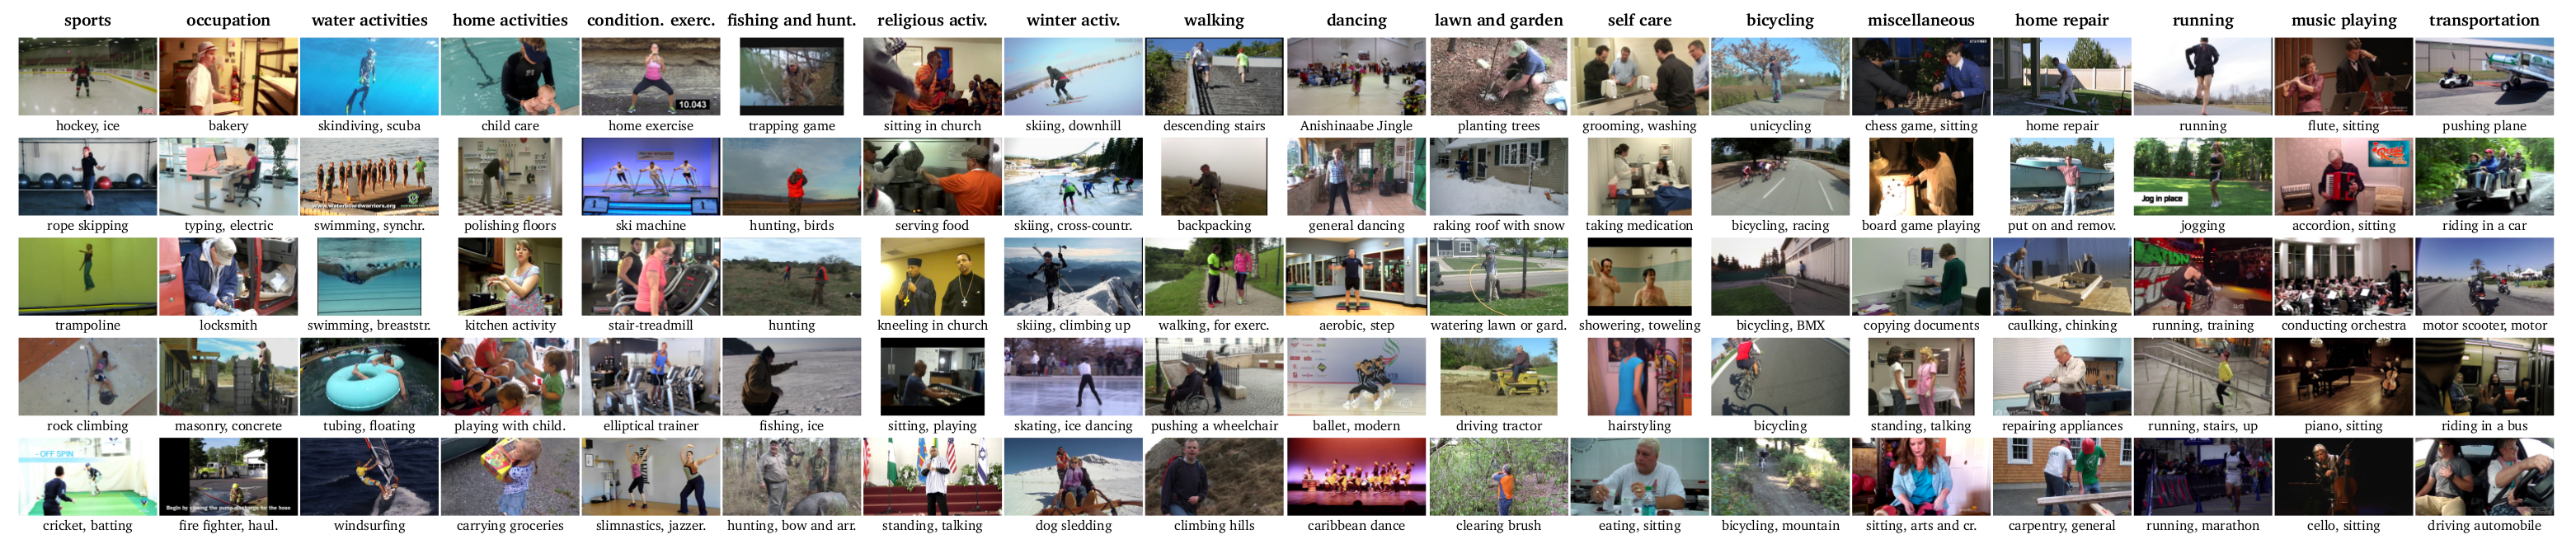
\includegraphics[width=1\linewidth]{proposal/mpii.png}
    \caption{\label{fig:mpii}MPII}
\end{figure}

在此外,我们还可以利用浙江大学图形学实验室的大型光场系统自己生成数据集。该系统含有一个球形阵列的相机,通过多相机的人体重建技术,可以获得人体的三维模型。

\begin{figure}[ht]
    \centering
    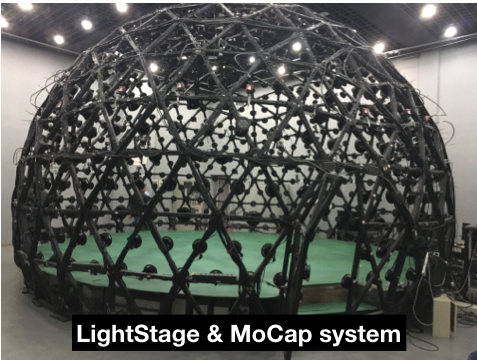
\includegraphics[width=.4\linewidth]{proposal/lightstage.jpg}
    \caption{\label{fig:light}光场系统}
\end{figure}

对于一般的室外场景,人们只能对其在图片上的关节坐标进行标注,而无法标出人体的三维坐标。因此如何获得室外图片的三维坐标是一个困难的问题,这也是三维人体姿态估计领域的一个挑战。
\subsection{人体检测}
在图像中检测出人体已经是一个比较成熟的技术了,可以在别人的工作的基础上进行改进,使其更适合我们的需要。

\subsection{二维人体姿态估计}
目前估计二维人体的姿态也比较成熟了,因为可以通过人标注许多的数据集,使用深度学习技术可以比较容易的学习到图片中的人体的二维关节坐标。

\subsection{三维人体姿态估计}
目前三维人体姿态估计仍是一个比较困难的问题,对于三维人体姿态估计问题,目前的方法主要分为两类:端到端法(end-to-end)\autocite{pavlakos2017coarse}和两步法(two-step)\autocite{zhou2016sparseness}。端到端法(end-to-end)\autocite{pavlakos2017coarse}是指对输入的图像或者视频通过一个卷积网络(ConvNet)的处理直接得到人体的三维姿态;而两步法(two-step)\autocite{zhou2016sparseness}通常是指先根据输入的图像或视频,提取出对应的二维人体姿态,再使用优化的方法或深度学习的方法得到人体的三维姿态。

使用端到端法的好处是可以充分利用图片的信息,因此得到的结果更加鲁棒。但是这样的训练数据是难以获得的,目前的图片到人体的三维姿态的数据大多来源于特定场景下,使用动作捕捉系统或者多相机阵列获得,无法泛化到一般场景下;而使用两步法的好处是不需要从图片到三维姿态的数据,可以两个步骤分别进行,显然,缺点是在估计三维姿态的时候无法利用到图片信息。

我们的工作会对两种方法都进行试验,然后进行比较,选择适合于我们的问题的方法。

\subsection{三维人体模型估计}
SMPL\autocite{loper2015smpl}是一种参数化表示的人体模型,这个模型从大量三维人体扫描数据中去学习人体的参数化表示,使得人们可以通过低维的参数去表示不通形状的人体模型。如\refFig{fig:smpl0}所示。
\begin{figure}[ht]
    \centering
    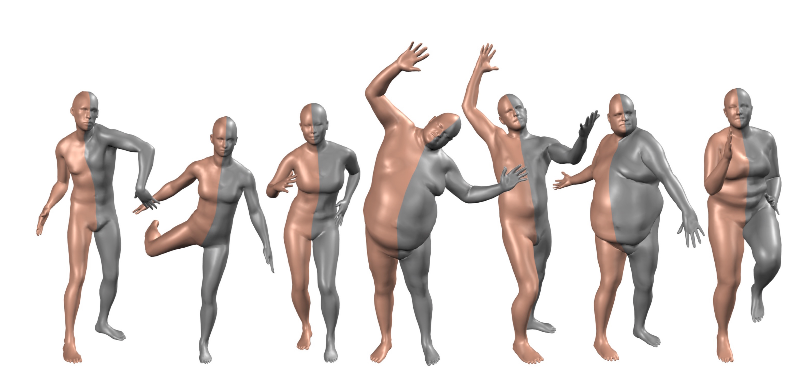
\includegraphics[width=1\linewidth]{proposal/smpl.png}
    \caption{SMPL\autocite{loper2015smpl}人体模型}\label{fig:smpl0}
\end{figure}
当下有一些文献认为仅仅用 3D 骨架的方法来描述 3D 姿态过于简单, Bogo等人\cite{bogo2016keep}提出了 SMPLify,一种基于优化的,从 14 个检测到的二维关节恢复SMPL 参数的方法。Bogo等人\cite{bogo2016keep}使用了优化的方法,将人体模型拟合到从图片中检测出来的二维人体关键点上。但是,由于加入了优化步骤,该方法不是实时的,每个图像需要 20-60 秒的时间进行处理。同时,由于从二维到三维的歧义性,他们在优化过程中加入了许多先验的知识,例如关节的角度的旋转范围,以及一个大量的姿势数据,使得得到的姿势接近数据库中的姿势。其部分结果如\refFig{fig:smpl}所示。 

\begin{figure}[ht]
    \centering
    \includegraphics[width=1\linewidth]{review/smplify.pdf}
    \caption{Keep it SMPLify\autocite{bogo2016keep}:通过拟合SMPL人体模型到图片的二维关键点上}\label{fig:smpl}
\end{figure}

我们的方法也会打算采用SMPL模型来对人体进行描述,通过结合人体模型的几何信息与深度学习方法得到的三维关节点信息,实现对人体姿态的更好的估计。

\section{可行性分析}
数据集方面,可以以开源的数据集为基础,再加上我们自己采集的人体数据。开源数据可以获取得到,在采集数据集上面,如何更好地使用光场系统进行重建,并得到我们需要的数据,还需要进一步工作。

在姿态估计方面,需要对目前已有的论文及模型进行复现,达到原始论文的效果,并能够迁移到我们的问题上。并在此基础上增加上我们的代码,完成人体姿态估计的整个流程。

在硬件方面,实验室有GPU可以使用,可以支持人体姿态估计任务的网络的训练。
